%# -*- coding: utf-8 -*-
% !TeX encoding = UTF-8 Unicode
% !TeX spellcheck = en_US
% !TeX TS-program = xelatex
%~ \XeTeXinputencoding "UTF-8"
% vim:ts=4:sw=4
%
% 以上设定默认使用 XeLaTex 编译,并指定 Unicode 编码,供 TeXShop 自动识别

\chapter{app-conv2dash}


\section{High Level Design}



\begin{enumerate}
  \item 使用 flowchart 将处理流程初步理清
  \item 使用 \href{http://www.cascading.org/}{Cascading}/MapReduce 实现系统
  \item 测试
\end{enumerate}


\subsection{介绍}

use hadoop to process multimedia contents and simulation

The main tasks we need to contruct the system are:

\begin{enumerate}
  \item transcode task:
  transcode the original media files (*.png, *.flac) to various resolution of the video files,
  generate the .mpd file for DASH

  \item emulation/simulation:
  how to select the parameters for a DASH adaptive algorithm

  \item result process:
  draw the figures?

\end{enumerate}


\subsection{整体结构}
图 \ref{fig:system} 是整个系统的运行框架。
首先,在模块 ``Media Transcode'' 中,用户需要对原始视频源处理,
输出若干解析度和比特率的视频。
这些处理过的视频资源作为输入数据,在 ``Simulation'' 中模拟DASH系统。
在模拟过程所收集到的数据被分析后,重新调整参数,做下次测试。
多轮循环后,输出结果。

\begin{figure}\centering
  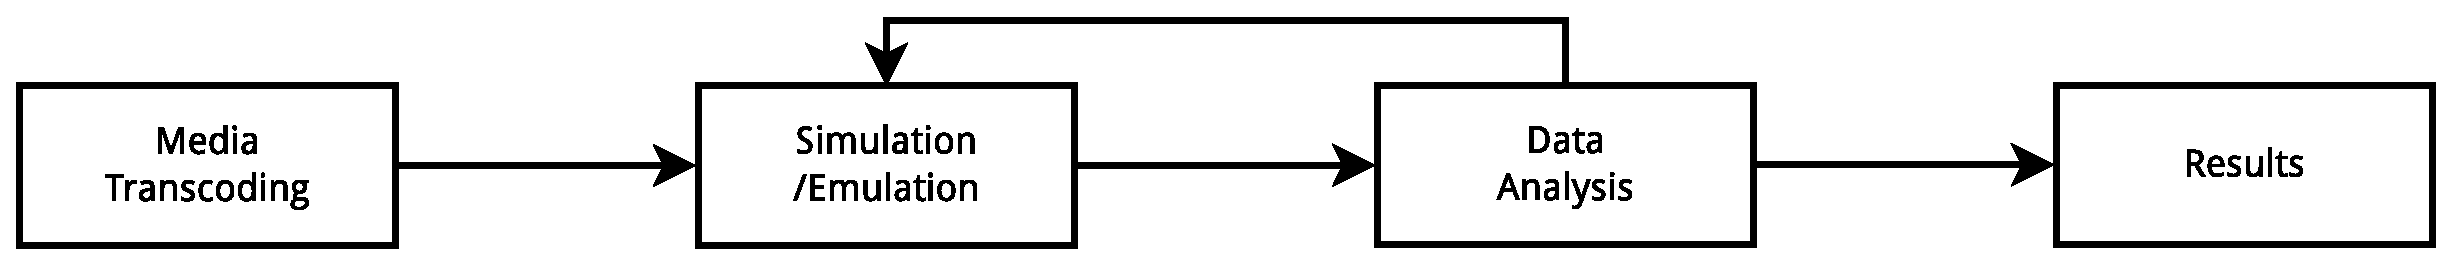
\includegraphics[width=0.9\textwidth]{figures-appconv2dash/flowchart-0-system.eps}
  \caption{The system.}\label{fig:system}
\end{figure}



\subsubsection{模拟参数}

\begin{figure}\centering
  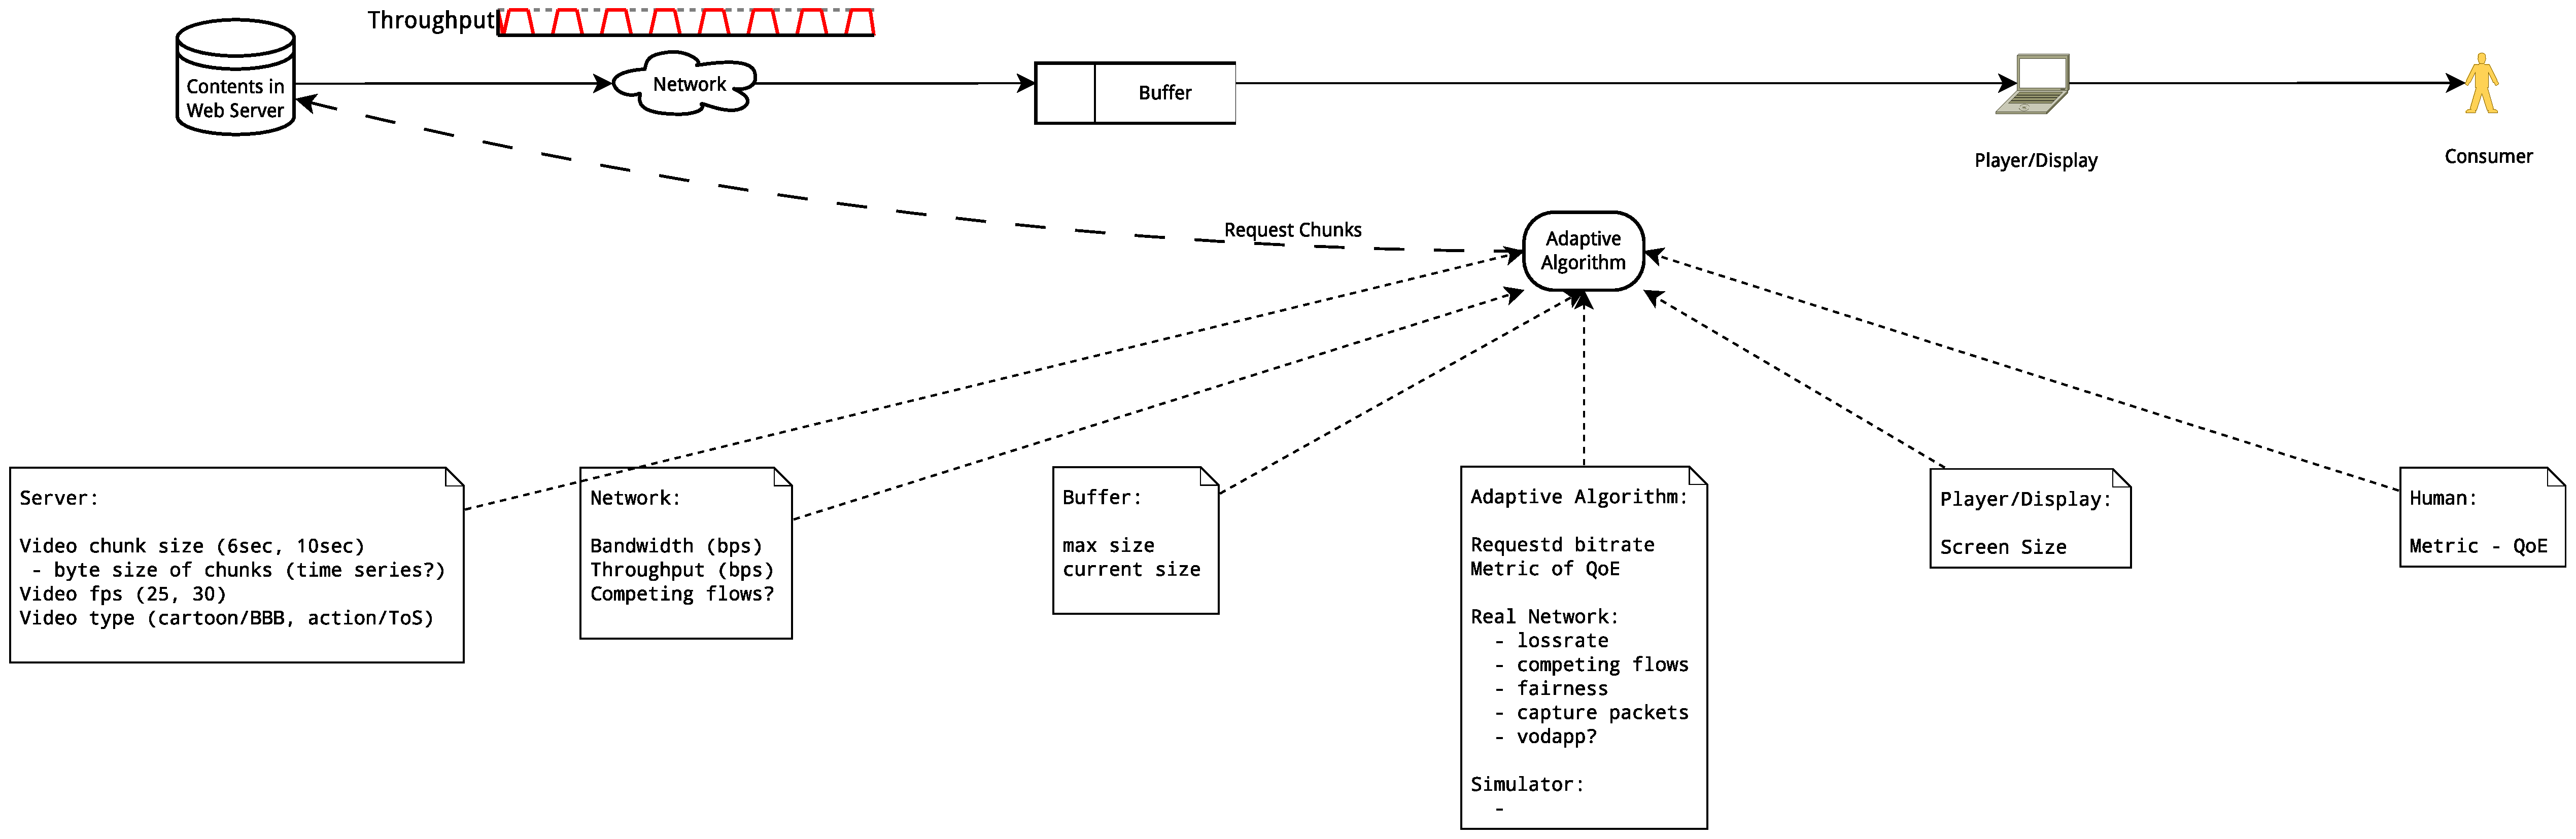
\includegraphics[width=1.1\textwidth]{figures-appconv2dash/dash-parameters.eps}
  \caption{\cnt{The metrics/parameters of the system}{系统参数/测量值}{}.}\label{fig:dashalgoparam}
\end{figure}



\begin{enumerate}
  \item How to evaluate the performance of one video streaming adaptive algorithm? (user metrics, network usages, fairness)
  \item What's the expected results?
  \item training the ML decision algorithm, by metrics(output), parameters(input);
  pre-select parameters for encoder (is it make sense for adaptive algorithm?)
\end{enumerate}




\subsection{用户接口}

用户一般有各种不同内容的视频文件,
需要将其转码到固定几种格式的输出。

基于用户使用习惯,可以将数据接口分为以下几类:

\begin{enumerate}
  \item 输入文件:作为Hadoop 应用程序输入参数的传递;文件的每一行是一个输入视频音频及其相关参数,用于生成一套各种码率的视频;可以在该输入文件中指定若干个视频音频源,输出是多个视频源的结果。
  \item 输出配置:输出是固定格式,包括压缩编码方式、解析度、比的率等;需要在 etc/transcode.conf 中配置
\end{enumerate}




\subsection{视频编码}

图 \ref{fig:vidtranscode} 是一个视频转换编码的流程图。
音频相对占用资源比较小,所以没有并行化。



%\textcolor[HTML]{0000FF}{This text will appear green-colored}

%\textcolor[HTML]{D7FE39}{This text will appear green-colored}


\definecolor{vidtransoriginfile}{HTML}{D7FE39}
\definecolor{vidtranstmpfile}{HTML}{EDE80F}
\definecolor{vidtransfinalfile}{HTML}{FFE985}
\definecolor{vidtransprocess}{HTML}{FEA93E}
\definecolor{vidtransfuncio}{HTML}{DADAFF}
\begin{figure}\centering
  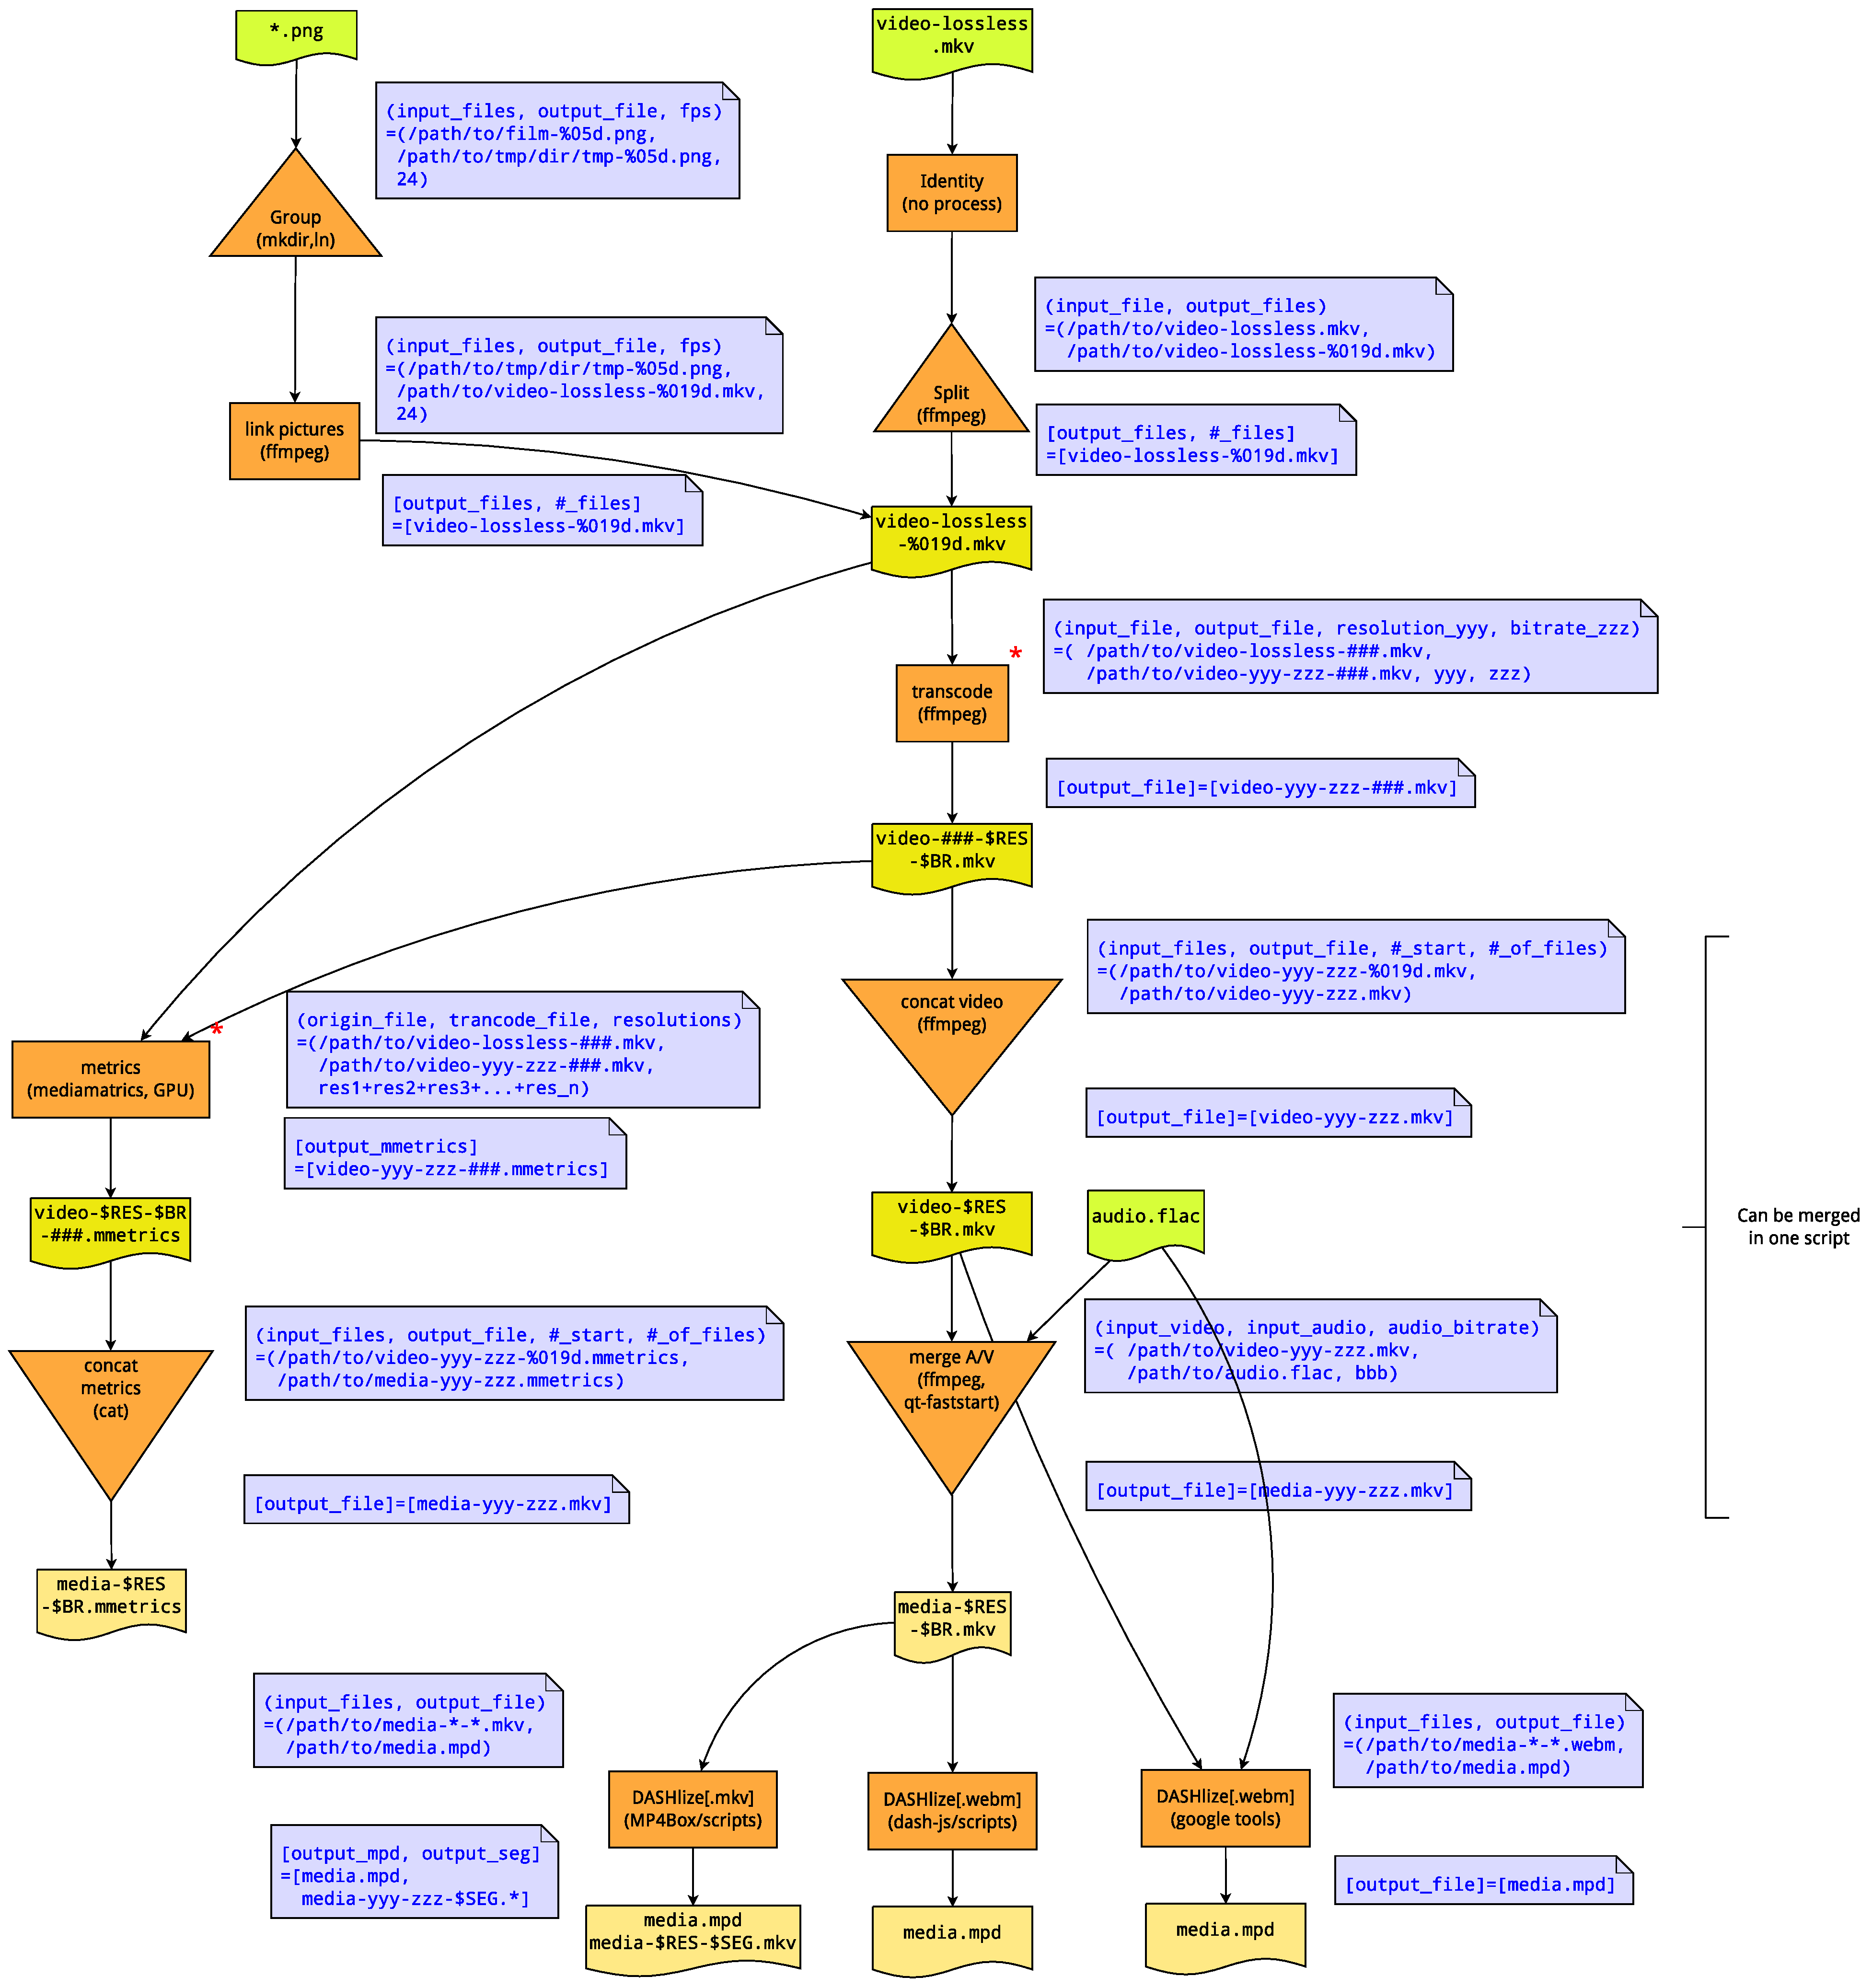
\includegraphics[width=1.1\textwidth]{figures-appconv2dash/flowchart-1-transcode.eps}
  \caption{Data flow for video transcoding.
    The text in \fcolorbox{black}{vidtransoriginfile}{this color} is the original input file.
    The text in \fcolorbox{black}{vidtranstmpfile}{this color} is the temp file.
    The text in \fcolorbox{black}{vidtransfinalfile}{this color} is the final output file.
    The text in \fcolorbox{black}{vidtransprocess}{this color} is process block.
    The text in \fcolorbox{black}{vidtransfuncio}{\textcolor[HTML]{0000FF}{this color}} is the input/output of one process block.
The process blocks signed by a \textcolor[HTML]{FF0000}{*} are the blocks cost most of the processing time.
  }\label{fig:vidtranscode}
\end{figure}



\subsubsection{DASH 化}
目前有三种转换的工具:

\begin{enumerate}
  \item Google tools (webm)

``Google tool'' 需要视频和音频分开处理,所以需要额外的步骤,参见 \ref{fig:googletoolmpd}

\begin{figure}\centering
  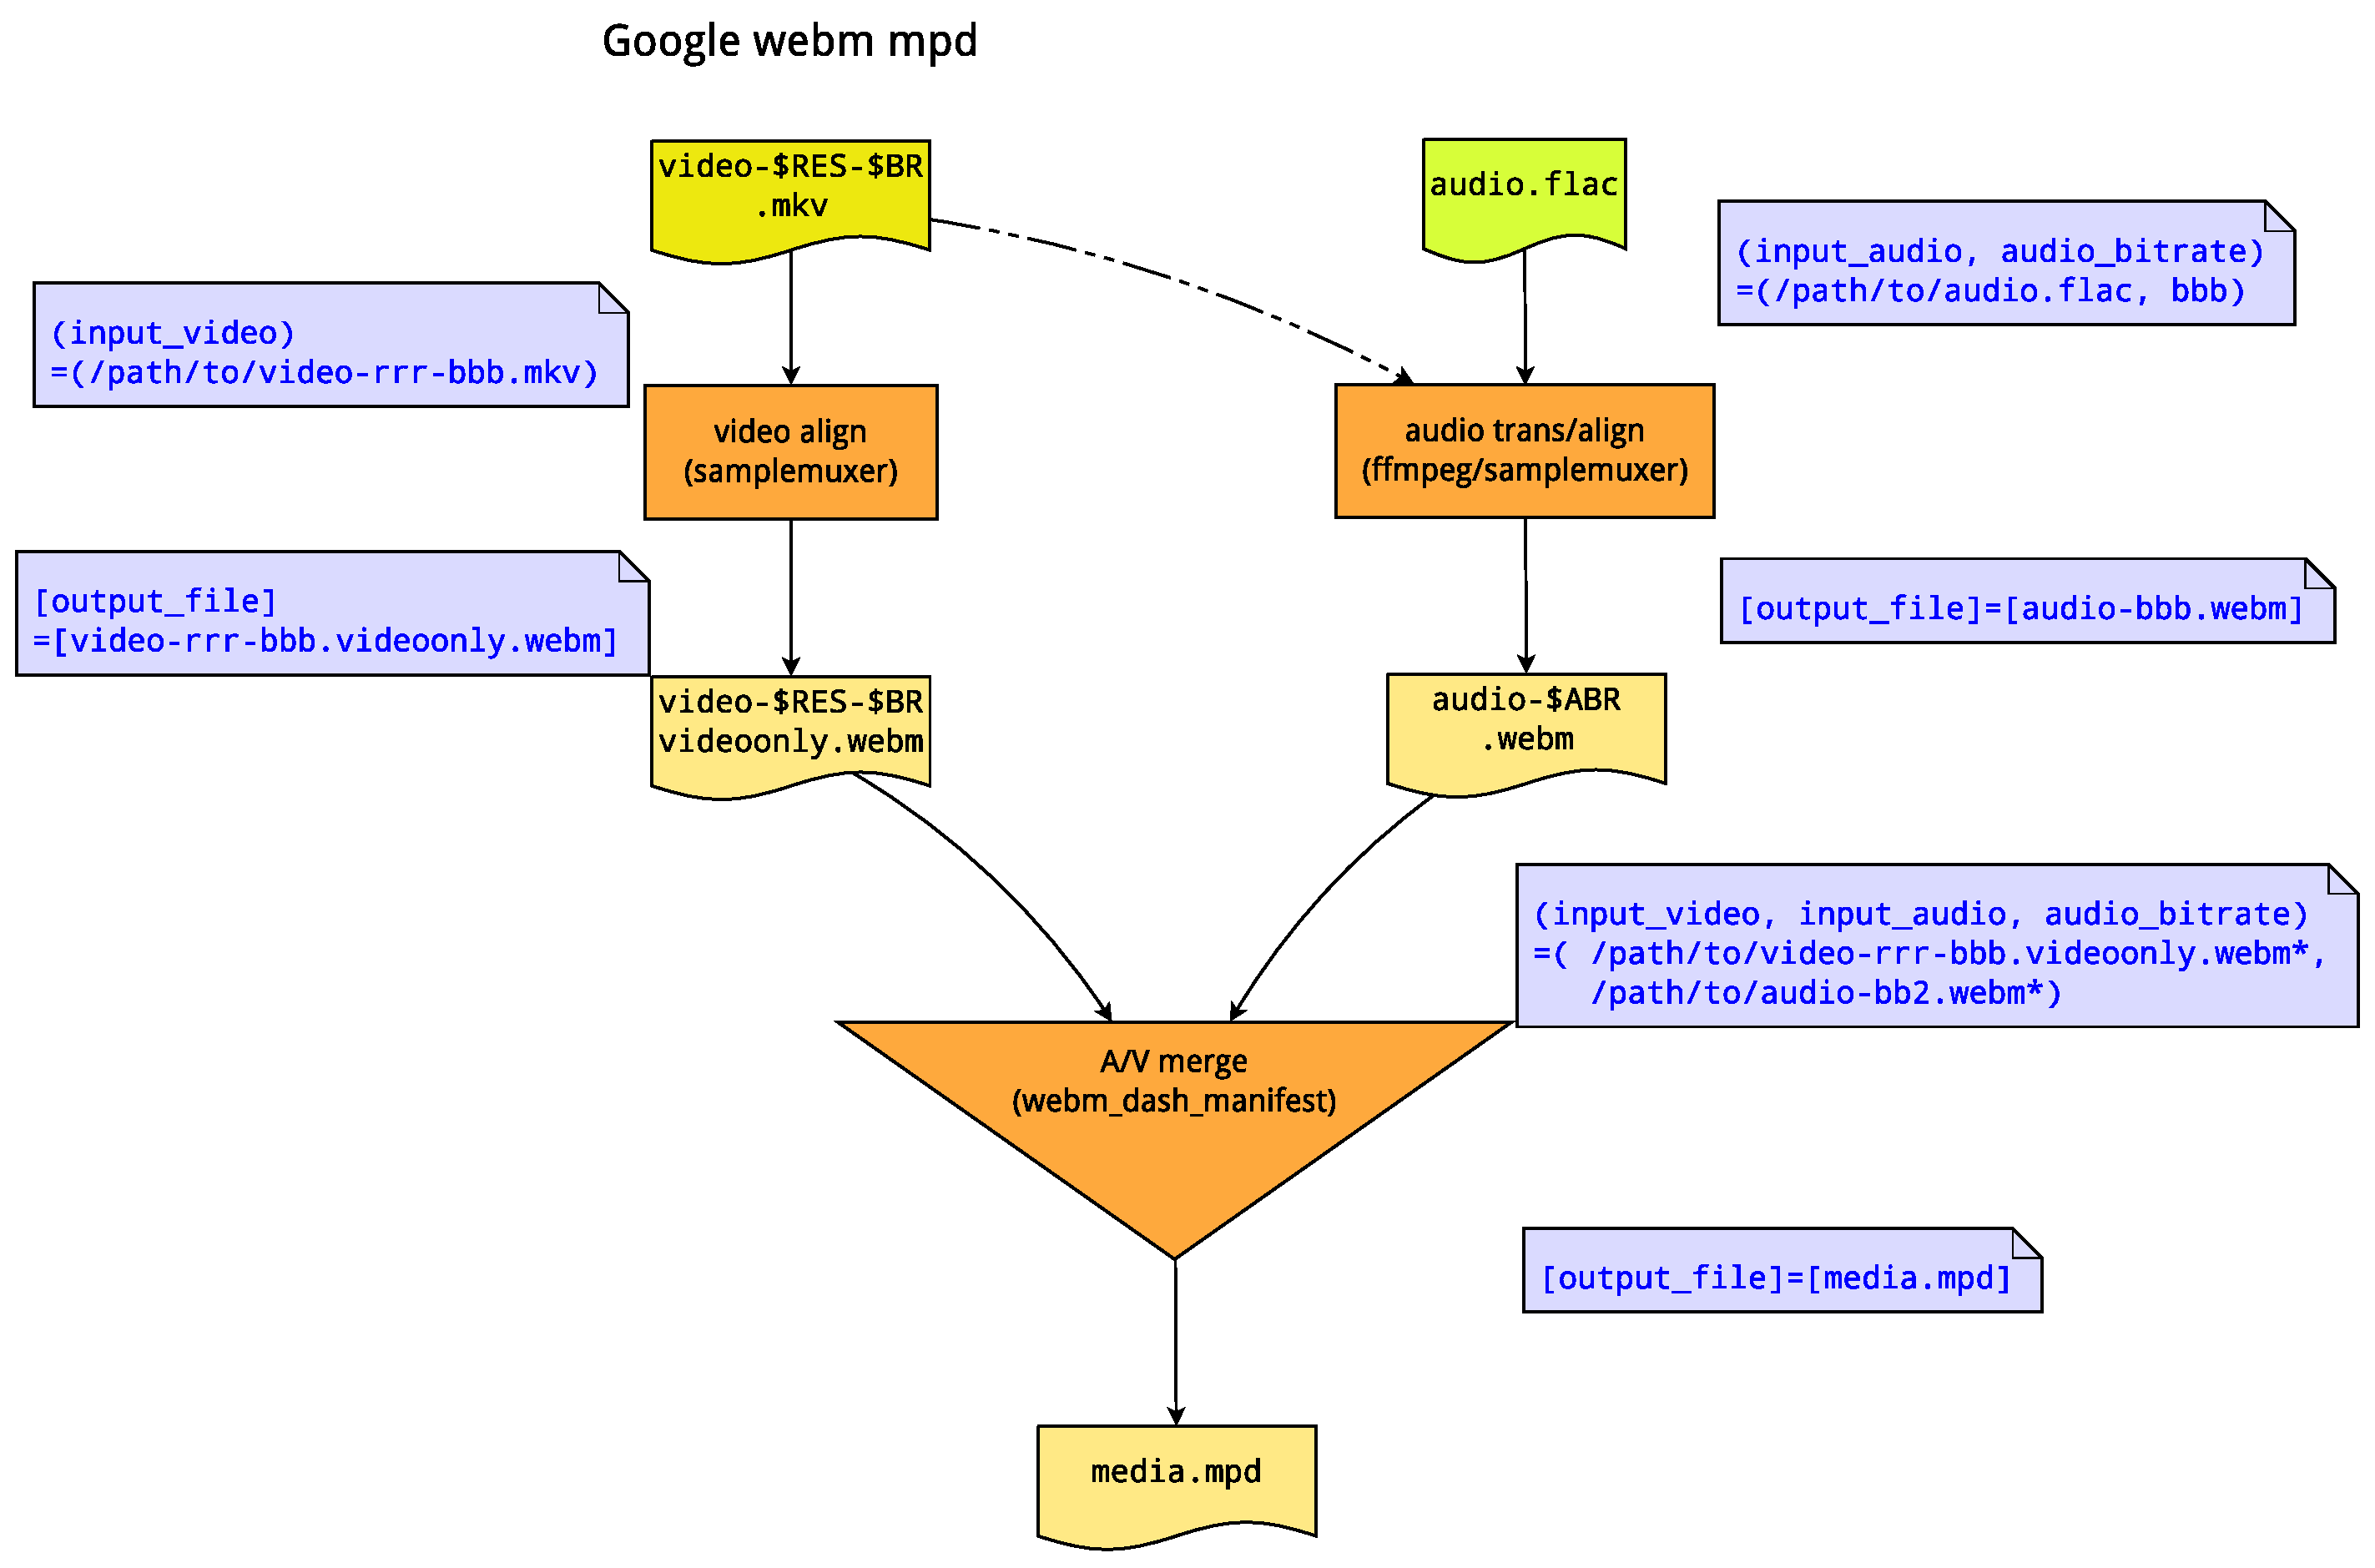
\includegraphics[width=0.9\textwidth]{figures-appconv2dash/flowchart-1-googletoolmpd.eps}
  \caption{Data flow for dashlize by google's tools.}\label{fig:googletoolmpd}
\end{figure}

\begin{lstlisting}[language=bash]
# video transcode
ffmpeg -i video-rrr-bbb.mkv \
    -vcodec libvpx -vb 3800k -s 1920x1080 \
    -keyint_min 150 -g 150 -sc_threshold 0 \
    -an -y video-rrr-bbb.videoonlytmp.mkv
# video align
samplemuxer -i video-rrr-bbb.videoonlytmp.mkv -o video-rrr-bbb.videoonly.mkv

# audio transcode
ffmpeg -i audio.flac -vn -acodec libvorbis -ab 256k -y audio-256k.tmp.webm
# audio align
samplemuxer -i audio-256k.tmp.webm -o audio-256k.webm \
    -output_cues 1 \
    -cues_on_audio_track 1 \
    -max_cluster_duration 5 \
    -audio_track_number 2
\end{lstlisting}

  \item {GPAC MP4Box (mp4)}

MP4Box 会分解文件,生成 mpd 配置文件,参见 \ref{fig:mp4boxmpd}

\begin{figure}\centering
  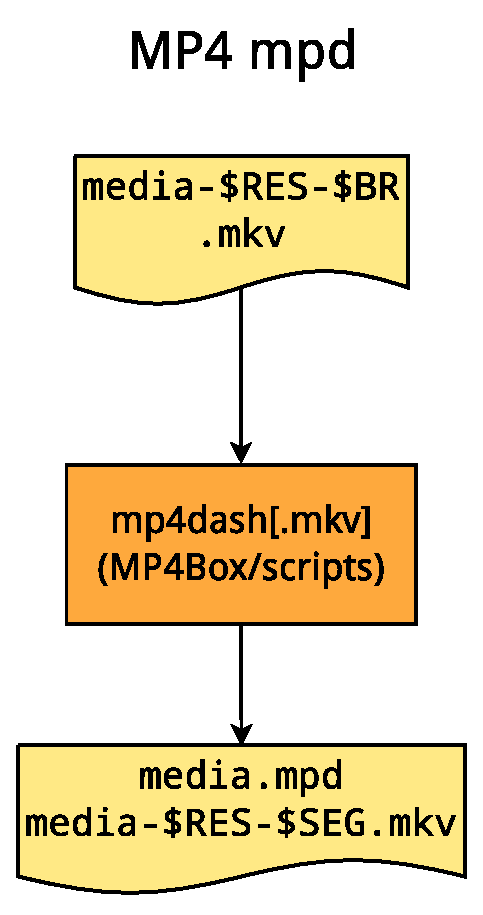
\includegraphics[width=0.3\textwidth]{figures-appconv2dash/flowchart-1-mp4boxmpd.eps}
  \caption{Data flow for dashlize by mp4box.}\label{fig:mp4boxmpd}
\end{figure}

参考命令行:
\begin{lstlisting}[language=bash]
SEGSEC=6
MP4Box -url-template -rap -frag $((500 * ${SEGSEC})) -dash $((1000 * ${SEGSEC})) -segment-name "prefix" "media-rrr-bbb.mkv"
\end{lstlisting}


  \item {dash.js (webm)}


dash.js 的是一个 Python 脚本,参见 \ref{fig:dashjsmpd}.

\begin{figure}\centering
  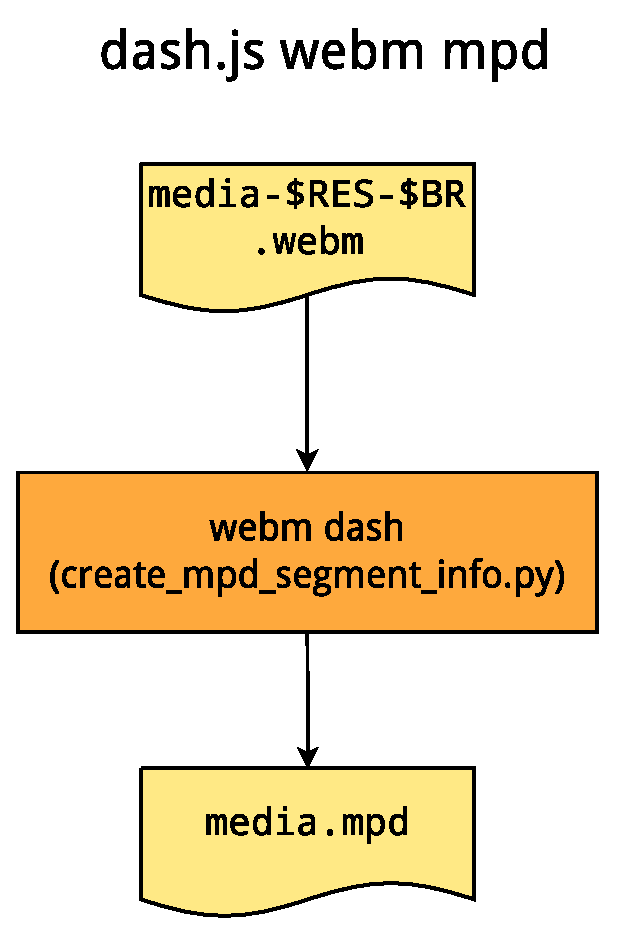
\includegraphics[width=0.3\textwidth]{figures-appconv2dash/flowchart-1-dashjsmpd.eps}
  \caption{Data flow for dashlize by dash.js.}\label{fig:dashjsmpd}
\end{figure}


参考命令行:
\begin{lstlisting}[language=bash]
SEGSEC=6
python dash-js-git/create_mpd_segment_info.py "media-rrr-bbb.webm" ${SEGSEC} $((${SEGSEC} * 2)) "" >> "media.mpd"
\end{lstlisting}

\end{enumerate}


\subsection{Emulation}

TODO






\section{Low Level Design}

Hadoop 中 streaming 模式下区分 key/value 的分节符缺省是 TAB;
也可以通过 \texttt{-D stream.map.output.field.separator=} 来设置。

\begin{itemize}
  \item \texttt{-D stream.map.output.field.separator} -- 设置 map 的输出中 key 和 value 的分隔符
  \item \texttt{-D stream.num.map.output.key.fields} -- 设置 map 的输出中区分 key部分 和 value部分 的分隔符的位置
  \item \texttt{-D map.output.key.field.separator} -- 设置 map 输出中 key 的子分割符
  \item \texttt{-D num.key.fields.for.partition} -- key 按照子分割符切割后,用于分桶 子key 所占的列数
        (使用 \texttt{-partitioner org.apache.hadoop.mapred.lib.KeyFieldBasedPartitioner} )
  \item \texttt{-D stream.reduce.output.field.separator} -- 设置 reduce 输出中 key 和 value 的分隔符
  \item \texttt{-D stream.num.reduce.output.key.fields} -- 设置 reduce 输出中 key部分 和 value部分 的分隔符的位置
\end{itemize}


\subsection{The Transcoding Module}

提供文件转码的功能,将无损视频和音频转换为指定解析度和比特率的多媒体文件和DASH .mpd 文件。

\textbf{问题}

\begin{itemize}
  \item \texttt{ffmpeg -f segment} 分解的文件块不是等 frame 个数,需要在最后附上各个分块的frame个数!
  \item 简化对用户接口。需要用户提供的参数可以缩减到:
    \begin{itemize}
      \item 视频文件类型(图片,视频)和路径
      \item 音频文件
      \item 分片大小
      \item 帧率(图片)
      \item 转码 分辨率-比特率 对(列表)
      \item 视频 matric 屏幕大小列表
    \end{itemize}
  如何设计接口可以让这些参数传递到下级?例如,转码才要用到的 分辨率-比特率 对(列表) 信息。
  针对不同视频比特率的对应的音频比特率如何获取?
  \item 其中音频文件是在任务的中间使用,可以通过配置文件设置,但这样会和用户输入``脱节'',输入参数和视频分开了,
  不容易管理使用。所以,将音频输入文件信息和视频输入信息放在一起输入,这样,程序需要一直传递音频信息直到所需要的地方。

  如果用户处理的时候,可以接受分片文件,包括音频视频分开,则可以不包含音频部分的处理。
\end{itemize}

\subsubsection{Interface of the link pictures/split processing}

使用 hadoop streaming 模式,
输入是含有需要处理的文件的列表。
对于源处理文件是视频单帧图片文件,文件名需要是顺序数字编号的格式;
而要提供 路径名format、分片大小(时间)、起始编号、文件个数、帧率 等五个参数作为输入参数。
输出文件为一系列分片视频文件。

\begin{enumerate}
  \item \textbf{map}
处理:
预先处理文件,
如果是单独视频文件,则分解视频文件,将分块文件名传送到下步做排序后获取各个块的frame大小,计算对应的起始frame编号送给 lossless 处理;
如果是图片,则输出目录下所有文件名,然后通过后面的shuffle排序后分组做无损压缩操作。


输入参数:
\begin{lstlisting}[language=bash]
<type> <audio_file> <video_file_fmt> <segsec> [<fps> <#start> <#files>]
# origpic "/path/to/audio1.flac" "/path/to/film-%05d.png"      6 24 1 1253
# origvid "/path/to/audio2.flac" "/path/to/video-lossless.mkv" 6
\end{lstlisting}


输出:
\begin{lstlisting}[language=bash]
<type> <path_in> <segsec> <audio_file> [<path_out> <fps>]
picgroup   <key> <audio_file> <vid_seg_file_name_out> <segsec> <fps> <frame_start_number>
processvid <key> <audio_file> <vid_seg_file_name_out> <segsec>
# picgroup   "/path/to/film-%05d.png"      "/path/to/audio1.flac" "/path/to/tmp/video-0000000000000000000.lossless.mkv" 6 24 0
# picgroup   "/path/to/film-%05d.png"      "/path/to/audio1.flac" "/path/to/tmp/video-0000000000000000001.lossless.mkv" 6 24 144
# processvid "/path/to/video-lossless.mkv" "/path/to/audio2.flac" "/path/to/tmp/video-0000000000000000001.lossless.mkv" 6
\end{lstlisting}

磁盘上生成对应的图片文件分组目录。

  \item \textbf{reduce}
处理:
将输入转换成无损压缩的分片视频文件。


输入参数:(前4列为key)
\begin{lstlisting}[language=bash]
<type> <path_in> <segsec> <audio_file> [<path_out> <fps>]
picgroup   <key> <audio_file> <vid_seg_file_name_out> <segsec> <fps> <frame_start_number>
processvid <key> <audio_file> <vid_seg_file_name_out> <segsec>
# picgroup   "/path/to/film-%05d.png"      "/path/to/audio1.flac" "/path/to/tmp/video-0000000000000000000.lossless.mkv" 6 24 0
# picgroup   "/path/to/film-%05d.png"      "/path/to/audio1.flac" "/path/to/tmp/video-0000000000000000001.lossless.mkv" 6 24 144
# processvid "/path/to/video-lossless.mkv" "/path/to/audio2.flac" "/path/to/tmp/video-0000000000000000001.lossless.mkv" 6
\end{lstlisting}

输出:
\begin{lstlisting}[language=bash]
<type> <serial#> <video_file> <resolution> <video_bps> <audio_file> <audio_bps>
# lossless 0 "/path/to/tmp/video-0000000000000000000.lossless.mkv"  320x180   315k "/path/to/audio1.flac" 64k
# lossless 0 "/path/to/tmp/video-0000000000000000000.lossless.mkv"  640x360   705k "/path/to/audio1.flac" 64k
# lossless 0 "/path/to/tmp/video-0000000000000000000.lossless.mkv"  853x480  1200k "/path/to/audio1.flac" 192k
# lossless 0 "/path/to/tmp/video-0000000000000000000.lossless.mkv" 1280x720  3200k "/path/to/audio1.flac" 256k
# lossless 0 "/path/to/tmp/video-0000000000000000000.lossless.mkv" 1920x1080 4200k "/path/to/audio1.flac" 256k
# lossless 144 "/path/to/tmp/video-0000000000000000001.lossless.mkv"  320x180   315k "/path/to/audio1.flac" 64k
\end{lstlisting}

磁盘上生成对应的视频分片文件。

视频解析度比特率和音频比特率列表从全局设置文件中读出。
\end{enumerate}


\subsubsection{Interface of the transcoding processing}

转码、串接视频、合并音频。

\begin{enumerate}
  \item \textbf{map}

处理:
将输入无损压缩的分片视频文件 转码成指定的分辨率-比特率 的视频文件。


输入参数:
\begin{lstlisting}[language=bash]
<type> <seq_frame> <video_file> <resolution> <video_bps> <audio_file> <audio_bps>
# lossless 0 "/path/to/tmp/video-0000000000000000000.lossless.mkv"  320x180 315k "/path/to/audio1.flac" 64k
# lossless 144 "/path/to/tmp/video-0000000000000000001.lossless.mkv"  320x180 315k "/path/to/audio1.flac" 64k
\end{lstlisting}

输出:(前2列为关键key,第3列作为排序key的一部分)
\begin{lstlisting}[language=bash]
concat  <video_destination> <transcode_file> <audio_file> <audio_bitrate>
# concat "/path/to/video-320x180-315k.mkv" "/path/to/tmp/video-320x180-315k-0000000000000000000.mkv" "/path/to/audio1.flac" 64k
# concat "/path/to/video-320x180-315k.mkv" "/path/to/tmp/video-320x180-315k-0000000000000000001.mkv" "/path/to/audio1.flac" 64k
\end{lstlisting}

\begin{lstlisting}[language=bash]
metricsv <transcode_file> <mmetrics_destination> <origin_file> <start_frame_number> <screen_resolution>
# metricsv "/path/to/video-320x180-315k.metricsv" "/path/to/tmp/video-320x180-315k-0000000000000000000.mkv" "/path/to/tmp/video-lossless-0000000000000000000.mkv" 0 1280x720
# metricsv "/path/to/video-320x180-315k.metricsv" "/path/to/tmp/video-320x180-315k-0000000000000000001.mkv" "/path/to/tmp/video-lossless-0000000000000000001.mkv" 144 1280x720
\end{lstlisting}

如果输出是 webm格式文件的化:(前3列为key,因为需要分布式处理,key越散越好)
\begin{lstlisting}[language=bash]
audioenc <transcode_file> <origin_file> <audio_bitrate> <mpd_destination>
# audioenc "/path/to/audio-256k.webm" "/path/to/audio.flac" 256k "/path/to/video.gwebm.mpd"
\end{lstlisting}


磁盘上生成对应的视频文件。

concat 类型的 resolution 和 bitrate 是用于 reduce 来做合并操作, 输出的 audio\_bitrate 是给下步做参数用。

下面的reduce处理, concat 主要是集合文件,所以必须以文件名排序(第3列),同时以 destination 为聚合文件名,
所以指定前3列为key,而key 的 partition 为前2列。Hadoop 中的表示是:

\begin{lstlisting}[language=bash]
    -D stream.num.map.output.key.fields=3 \
    -D num.key.fields.for.partition=2 \
\end{lstlisting}

metrics 的记录为了能够打乱顺序(以便负载均衡),原有的 type,destination,trans 被设置为 type,trans,destination。

  \item \textbf{reduce -- concat}

处理:
针对 concat 类型的数据,在所有数据收集齐后,做串接成完整视频的操作.

这时,因为需要支持三种不同工具的 DASH 化操作,需要分开完成相关准备工作。
对于MP4Box和dash.js的工具,需要的输入文件是A/V合并后的文件,所以还需等待后满操作完成后再做。

对于 google tools 是需要 A/V分开的 webm(mp4不支持) 文件,所以在串接视频文件后,需要立即进行,所以在这里需要发出
相关请求(dashwebmgmerge)。
另外,因为音频文件需要单独编码,所以在此步之前发出音频编码指令,在本步另外一个函数平级处理,然后同时也输出 dashwebmgmerge,这样下步可以做生成 mpd 文件的操作。

对于其他两种DASH工具,还需要合并音频。

输入参数:(前2列为关键key,第3列作为排序key的一部分)
\begin{lstlisting}[language=bash]
<type> <video_destination> <transcode_file> <audio_file> <audio_bitrate>
# concat "/path/to/video-320x180-315k.mkv" "/path/to/tmp/video-320x180-315k-0000000000000000001.mkv" "/path/to/audio1.flac" 64k
\end{lstlisting}


输出:(前2列为关键key,第3列作为排序key的一部分)
\begin{lstlisting}[language=bash]
dashwebmgmerge <mpd_destination> <mediatype> <transcode_file>
# dashwebmgmerge "/path/to/video.gwebm.mpd" video "/path/to/video-320x180-315k.mkv"
\end{lstlisting}

输出:
\begin{lstlisting}[language=bash]
dashmpd <mpd_destination> <mediatype> <transcode_file>
# dashmpd "/path/to/video.mpd" av "/path/to/video-320x180-315k.mkv"
\end{lstlisting}

磁盘上生成对应的视频文件。

  \item \textbf{reduce -- metricsv}

处理:

使用 mediamatrics 的 \texttt{-b <start\_frame\_number>} 设置各个分块的起始 frame 号。

输入参数:(前3列为key,因为需要分布式处理,key越散越好)
\begin{lstlisting}[language=bash]
metricsv <mmetrics_destination> <transcode_file> <origin_file> <start_frame_number> <screen_resolution>
# metricsv "/path/to/video-320x180-315k.metricsv" "/path/to/tmp/video-320x180-315k-0000000000000000000.mkv" "/path/to/tmp/video-lossless-0000000000000000000.mkv" 0 1280x720
# metricsv "/path/to/video-320x180-315k.metricsv" "/path/to/tmp/video-320x180-315k-0000000000000000001.mkv" "/path/to/tmp/video-lossless-0000000000000000001.mkv" 144 1280x720
\end{lstlisting}


输出:
\begin{lstlisting}[language=bash]
metricsconcat <mmetrics_destination> <mediatype> <mmetrics_file>
# metricsvconcat "/path/to/video-320x180-315k.metricsv" txt "/path/to/tmp/video-320x180-315k-0000000000000000000.1920x1080.metricsv"
# metricsvconcat "/path/to/video-320x180-315k.metricsv" txt "/path/to/tmp/video-320x180-315k-0000000000000000001.1920x1080.metricsv"
\end{lstlisting}

磁盘上生成对应的视频文件、分片.metricsvideo 文件。

该文件是属于分片视频文件的,下一步需要在所有数据收集完后,进行合并。


  \item \textbf{reduce -- audioenc}

处理:
对音频做编码处理。


输入参数:(前3列为key,因为需要分布式处理,key越散越好)
\begin{lstlisting}[language=bash]
audioenc <transcode_file> <origin_file> <mpd_destination> <audio_bitrate>
# audioenc "/path/to/audio-256k.webm" "/path/to/audio.flac" "/path/to/video.gwebm.mpd" 256k
\end{lstlisting}


输出:(前2列为关键key,第3列作为排序key的一部分)
\begin{lstlisting}[language=bash]
dashwebmgmerge <mpd_destination> <mediatype> <transcode_file>
# dashwebmgmerge "/path/to/video.mpd" audio "/path/to/audio-256k.webm"
\end{lstlisting}

磁盘上生成对应的音频文件。

\end{enumerate}



\subsubsection{Interface of the metrics merging processing}
将 .metricsvideo 文件合并。

指定 reducer 个数为文件个数?


\begin{enumerate}
  \item \textbf{map}
NONE


  \item \textbf{reduce -- metricsvconcat}
处理:

输入参数:(前2列为关键key,第3,4列作为排序key的一部分)
\begin{lstlisting}[language=bash]
metricsvconcat <mmetrics_destination> <mediatype> <mmetrics_file>
# metricsvconcat "/path/to/video-320x180-315k.metricsvideo" txt "/path/to/tmp/video-320x180-315k-0000000000000000000.1920x1080.metricsvideo"
\end{lstlisting}

输出:
/path/to/video-320x180-315k.metricsvideo

磁盘上生成对应合并了的 \texttt{.metricsvideo} 文件。

这里是聚合所有文件,所以文件需要排序(前2列),聚合文件为第1列,所以设置:

\begin{lstlisting}[language=bash]
    -D stream.num.map.output.key.fields=2 \
    -D num.key.fields.for.partition=1 \
\end{lstlisting}




  \item \textbf{reduce -- dashwebmgmerge}
处理:
使用 google tools 的dash工具处理。
需要合并同样 destination 的视频/音频文件。


输入参数:(前2列为关键key,第3,4列作为排序key的一部分)
\begin{lstlisting}[language=bash]
dashwebmgmerge <mpd_destination> <mediatype> <transcode_file>
# dashwebmgmerge "/path/to/video.mpd" video "/path/to/video-320x180-315k.mkv"
\end{lstlisting}

输出:

\texttt{.mpd} 文件。



  \item \textbf{reduce -- dashmpd}
处理:
使用 dash mpd 工具处理。这里可以使用 MP4Box 和 dash.js 的。

输入参数:(前2列为关键key,第3,4列作为排序key的一部分)
\begin{lstlisting}[language=bash]
dashmpd <mpd_destination> <mediatype> <transcode_file>
# dashmpd "/path/to/video.mpd" av "/path/to/video-320x180-315k.mkv"
\end{lstlisting}

输出:

\texttt{.mp4box.mpd},\texttt{.dashjs.mpd} 文件(以及 dash 分片文件).


\end{enumerate}



\subsection{Simulation Emulation}
TBD

\subsection{Data Analysis}
TBD











\section{Implementation}

\subsection{The structure of the working directory}

\begin{itemize}
  \item \texttt{etc}: 一些和系统相关的配置
    \begin{itemize}
      \item \texttt{transcode.conf} 文件转码的一些配置,包括解析度,比特率、转码格式(x264,webm)等。
    \end{itemize}
  \item \texttt{bin}: 编译好的运行程序
  \item \texttt{lib}: 程序依赖库
  \item \texttt{data}: 使用的数据/结果
    \begin{itemize}
      \item \texttt{input}: 原始输入数据
      \item \texttt{output}: 输出数据/结果
      \item \texttt{buffer}: 中间结果
        \begin{itemize}
          \item \texttt{hdfs}: hadoop HDFS 使用的目录(如果有)
        \end{itemize}
  \end{itemize}
\end{itemize}


\subsection{Speed}


\subsubsection{测试方法}

为了对比单机和分布式速度上的提速,可以分别测试在单线程和多线程配置下的速度。

\begin{itemize}
  \item 单节点上单进程、ffmpeg 配置为单线程
  \item 单节点上单进程、ffmpeg 配置为多线程(3线程)
  \item 单节点上多进程(3进程)、ffmpeg 配置为单线程
  \item 单节点上多进程(3进程)、ffmpeg 配置为多线程(3线程)
  
\end{itemize}





以下是
在 i5-3360M 2核,4线程,16G RAM 机器上;
内存消耗小于4G.

\subsubsection{test 1}
webm

HDFF\_TRANSCODE\_RESOLUTIONS=320x180+315k+64k,640x360+500k+64k

HDFF\_SCREEN\_RESOLUTIONS=320x180


sintel trailer, png files, trancode, mediametric
\begin{lstlisting}[language=bash]
sh1 -- 203
hadoop -- 282
\end{lstlisting}


sintel trailer, 1080p mkv files, trancode, mediametric
\begin{lstlisting}[language=bash]
sh1 -- 241
hadoop -- 318
\end{lstlisting}


sintel trailer, png files + 1080p mkv file, trancode, mediametric
\begin{lstlisting}[language=bash]
sh1 -- 424
hadoop -- 516
\end{lstlisting}


\subsubsection{test 2}
webm

HDFF\_TRANSCODE\_RESOLUTIONS=320x180+315k+64k,640x360+500k+64k

HDFF\_SCREEN\_RESOLUTIONS=320x180


sintel trailer, png files
\begin{lstlisting}[language=bash]
1 process, 1 thread
[run-sh1.sh] Cost time: total=326 seconds
    stage1=57(m=0,r=57) seconds
    stage2=268(m=163,r=105) seconds
    stage3=1(m=0,r=1) seconds


1 process, 3 threads
[run-sh1.sh] Cost time: total=288 seconds
    stage1=51(m=1,r=50) seconds
    stage2=237(m=117,r=120) seconds
    stage3=0(m=0,r=0) seconds


3 processes, 1 threads
[run-sh1.sh] Cost time: total=211 seconds
    stage1=41(m=0,r=41) seconds
    stage2=169(m=90,r=79) seconds
    stage3=1(m=0,r=1) seconds


3 processes, 3 threads
[run-sh1.sh] Cost time: total=195 seconds
    stage1=42(m=1,r=41) seconds
    stage2=152(m=78,r=74) seconds
    stage3=1(m=0,r=1) seconds


auto: 3 processes, 2 threads
[run-sh1.sh] Cost time: total=226 seconds
    stage1=48(m=1,r=47) seconds
    stage2=177(m=89,r=88) seconds
    stage3=1(m=0,r=1) seconds
[run-sh1.sh] Cost time: total=211 seconds
    stage1=40(m=1,r=39) seconds
    stage2=171(m=92,r=79) seconds
    stage3=0(m=0,r=0) seconds
[run-sh1.sh] Cost time: total=229 seconds
    stage1=45(m=1,r=44) seconds
    stage2=183(m=96,r=87) seconds
    stage3=1(m=0,r=1) seconds


4 processes, 4 threads
[run-sh1.sh] Cost time: total=225 seconds
    stage1=47(m=1,r=46) seconds
    stage2=177(m=90,r=87) seconds
    stage3=1(m=0,r=1) seconds

# pic
palmetto, user, 21 processes, 7 threads
from /newscratch
[run-sh1.sh] config:
    HDFF_NUM_CLONE=21
    OPTIONS_FFM_GLOBAL= -threads 7
[run-sh1.sh] Cost time: total=870 seconds
    stage1=828(m=312,r=516) seconds
    stage2=41(m=17,r=24) seconds
    stage3=1(m=0,r=1) seconds

from /home
[run-sh1.sh] config:
    HDFF_NUM_CLONE=21
    OPTIONS_FFM_GLOBAL= -threads 7
[run-sh1.sh] Cost time: total=68 seconds
    stage1=37(m=1,r=36) seconds
    stage2=30(m=17,r=13) seconds
    stage3=1(m=0,r=1) seconds


# sintel
[run-sh1.sh] config:
    HDFF_NUM_CLONE=16
    OPTIONS_FFM_GLOBAL= -threads 0
[run-sh1.sh] Cost time: total=157269 seconds
    stage1=12840(m=4307,r=8533) seconds
    stage2=144311(m=4543,r=139678) seconds
    stage3=1(m=1,r=207) seconds


# tear of steel
[run-sh1.sh] config:
    HDFF_NUM_CLONE=16
    OPTIONS_FFM_GLOBAL= -threads 0
[run-sh1.sh] Cost time: total=47255 seconds
    stage1=2177(m=636,r=1541) seconds
    stage2=448833(m=2826,r=42057) seconds
    stage3=1(m=0,r=159) seconds


# BBB, no screen metrics
[run-sh1.sh] config:
    HDFF_NUM_CLONE=16
    OPTIONS_FFM_GLOBAL= -threads 0
[run-sh1.sh] Cost time: total=3912 seconds
    stage1=1995(m=437,r=1558) seconds
    stage2=1902(m=1798,r=104) seconds
    stage3=15(m=0,r=15) seconds

# BBB, with screen metrics
[run-sh1.sh] config:
    HDFF_NUM_CLONE=16
    OPTIONS_FFM_GLOBAL= -threads 0
[run-sh1.sh intercept] Cost time: total=84747 seconds
    stage1=1995(m=437,r=1558) seconds
    stage2=82554(m=1798,r=80756) seconds
    stage3=1(m=0,r=198) seconds


# elephent, with screen metrics
[run-sh1.sh] config:
    HDFF_NUM_CLONE=16
    OPTIONS_FFM_GLOBAL= -threads 0
[run-sh1.sh intercept] Cost time: total=107550 seconds
    stage1=1247(m=295,r=952) seconds
    stage2=106168(m=1775,r=104393) seconds
    stage3=1(m=1,r=134) seconds


\end{lstlisting}




